\chapter{クラスの例}
この回はクラスの例を示す。
\section{例の概要}
図\ref{color}はここで示す例の表示画面である。
\begin{figure}[ht]
 \begin{center}
  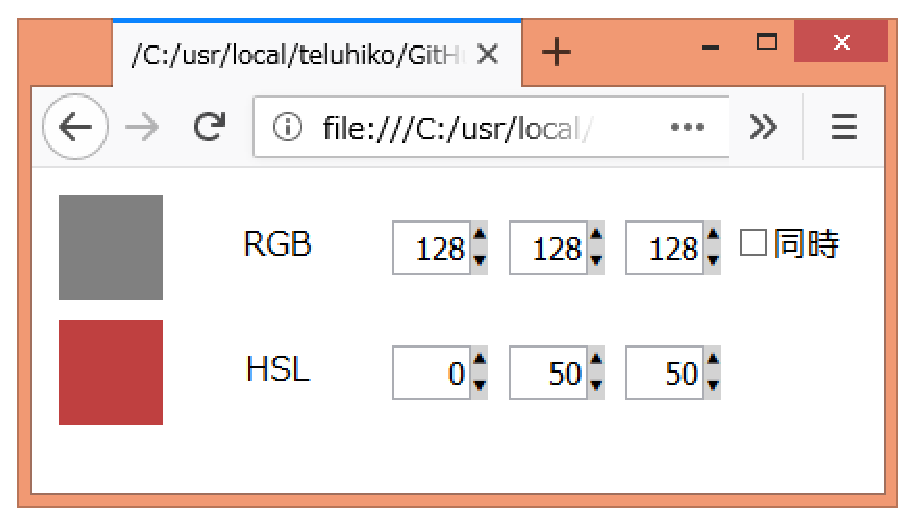
\includegraphics[width=0.5\textwidth]{13Ex.eps}
 \end{center}
 \caption{色の指定を見る}\label{color}
\end{figure}
この例では上下2行のテキストボックスで指定された色を左側の正方形の部分で
示す。上はRGB形式で、下はHSL\footnote{W3CのCSS Color Module Level
3\texttt{https://www.w3.org/TR/2011/REC-css3-color-20110607/}を参照のこ
と}形式で色を指定することができる。色を変える操作は次のとおりである。
\begin{itemize}
 \item それぞれのテキストボックスの値は▲をクリックすると増加し、▼をクリッ
       クすると1ずつ減少する。シフトキーを押しながらクリックすると5ずつ
       変化する。
 \item RGB形式の値は$0\sim255$の間で変化する。上限または下限の範囲を超え
       る場合は上限または下限の値にのままである。一番右のチェックボックスを
       チェックすると3つの値が同時に増減する。
 \item HSL形式の値は一番左(H--色相)が$0\sim359$の間で循環して変化し、残
       りの2つは$0\sim100$の間で変化する。
\end{itemize}
\section{ソースコード}
\subsection{HTMLファイル}
次のリストはHTMLファイルのものである。
\LISTN{13Ex.html}{1}{last}{\normalsize}
 \section{ユーザーインターフェイス}
 次のリストはユーザーインターフェイスのクラスを定義するものである。
\LISTN{13UI.js}{1}{5}{\normalsize}
\LISTN{13UI.js}{6}{10}{\normalsize}
\LISTN{13UI.js}{11}{43}{\normalsize}
\LISTN{13UI.js}{44}{49}{\normalsize}
\LISTN{13UI.js}{50}{58}{\normalsize}
\LISTN{13UI.js}{59}{65}{\normalsize}
\LISTN{13UI.js}{66}{121}{\normalsize}
\LISTN{13UI.js}{122}{last}{\normalsize}
 \section{ユーザーインターフェイスを引用するJavaScriptファイル}
 次のリストはユーザーインターフェイスを利用して、色の変化を見えるように
 するものである。
 \LISTN{13Ex.js}{1}{last}{\normalsize}
 